% COPSS Presidents' Award — Laureates (1981–2026)
% Compact tabular layout mirroring abel_prize_laureates_beamer.tex
% 46 laureates, one per year. Cross-award honors annotated in Field column.
% Compile with: xelatex copss_laureates_beamer.tex
\documentclass[aspectratio=169,9pt]{beamer}

\usetheme{default}\usecolortheme{default}
\setbeamertemplate{navigation symbols}{}
\setbeamertemplate{footline}{%
  \hfill{\tiny\color{mutedgray}\insertframenumber/\inserttotalframenumber}\hspace*{6pt}\vspace{4pt}%
}
\newcommand{\framesubject}{}
\setbeamertemplate{frametitle}{%
  \vspace{8pt}%
  \centering
  {\large\bfseries\color{copssclr}COPSS 会长奖 · \insertframetitle}\\[3pt]
  \textcolor{copssbg}{\rule{0.95\textwidth}{0.6pt}}%
  \vspace{-6pt}%
}

\usepackage{fontspec}\usepackage{xeCJK}
\setCJKmainfont{PingFang SC}[BoldFont=PingFang SC Semibold]
\setCJKsansfont{PingFang SC}
\setmainfont{Helvetica Neue}[BoldFont=Helvetica Neue Bold]
\setsansfont{Helvetica Neue}
\usepackage{booktabs}\usepackage{array}\usepackage{tikz}\usepackage{amssymb}
\usepackage{colortbl}\usepackage{graphicx}\usepackage{fontawesome5}

\definecolor{headerblue}{RGB}{41,65,122}
\definecolor{yearcolor}{RGB}{150,40,90}
\definecolor{fieldcolor}{RGB}{30,100,60}
\definecolor{mutedgray}{RGB}{100,100,100}
\definecolor{slidebg}{RGB}{250,252,255}
\definecolor{copssclr}{RGB}{33,102,172}     % 统计蓝
\definecolor{copssbg}{RGB}{222,235,250}     % 浅蓝底
\definecolor{fieldsclr}{RGB}{41,65,122}
\definecolor{abelclr}{RGB}{150,40,90}
\definecolor{wolfclr}{RGB}{180,120,0}
\definecolor{chernclr}{RGB}{15,110,92}
\definecolor{nobelclr}{RGB}{176,141,45}
\setbeamercolor{background canvas}{bg=slidebg}

% Award badges (cross-award annotation)
\newcommand{\fieldsbadge}{\textsuperscript{\normalfont\tiny\color{fieldsclr}$\blacklozenge$\kern-0.5pt F}}
\newcommand{\wolfbadge}{\textsuperscript{\normalfont\tiny\color{wolfclr}$\bigstar$\kern-0.5pt W}}
\newcommand{\chernbadge}{\textsuperscript{\normalfont\tiny\color{chernclr}$\blacksquare$\kern-0.5pt C}}
\newcommand{\gaussbadge}{\textsuperscript{\normalfont\tiny\color{copssclr}$\blacklozenge$\kern-0.5pt G}}

% Chinese name suffix
\newcommand{\cn}[1]{\newline{\scriptsize\color{mutedgray}#1}}
% #1=Name(+badges) #2=Year #3=Birth-Death #4=Nationality #5=Institution #6=Field
\newcommand{\lrow}[6]{%
  {\bfseries\color{copssclr}#1} & {\color{yearcolor}#2} & {#3} & {#4} & {\scriptsize #5} & {\scriptsize\color{fieldcolor}#6} \\[2.5pt]
}

\begin{document}

\begin{frame}[plain]
\begin{tikzpicture}[remember picture, overlay]
  \fill[copssclr!2] (current page.north west) rectangle (current page.south east);
  \fill[copssclr!6] (current page.north west) ++(1.55,-1.35) circle (2.45cm);
  \fill[copssclr!8] (current page.south east) ++(-1.9,1.45) circle (2.70cm);
  \node[anchor=center, font=\fontsize{18}{24}\selectfont\bfseries, text=copssclr]
    at ([yshift=2.80cm]current page.center) {COPSS 会长奖：统计学界的最高礼赞（1981–2026）};
  \node[anchor=center, font=\fontsize{11}{15}\selectfont, text=mutedgray]
    at ([yshift=1.60cm]current page.center) {COPSS Presidents' Award（考普斯会长奖）\enspace·\enspace 全 46 位得主};
  \draw[copssclr!50, line width=1.2pt] ([yshift=0.90cm, xshift=-5.0cm]current page.center)
    -- ([yshift=0.90cm, xshift=5.0cm]current page.center);
  \node[anchor=center, font=\fontsize{9}{12}\selectfont\bfseries, text=mutedgray]
    at ([yshift=0.20cm]current page.center) {与菲尔兹·沃尔夫·阿贝尔·陈省身奖无交叉；Donoho 另获高斯奖 2018 与邵逸夫奖 2013};
  \node[anchor=center] at ([yshift=-1.90cm]current page.center) {
    \begin{tikzpicture}[scale=1]
      \node[inner sep=0pt] at (-4.88,0.75) {
        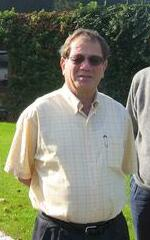
\includegraphics[width=0.6cm,height=0.7cm,keepaspectratio]{images/peterjbickel.jpg}
      };
      \node[inner sep=0pt] at (-4.22,0.75) {
        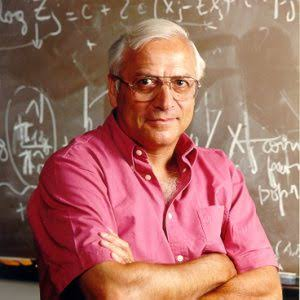
\includegraphics[width=0.6cm,height=0.7cm,keepaspectratio]{images/stephenfienberg.jpg}
      };
      \node[inner sep=0pt] at (-3.58,0.75) {
        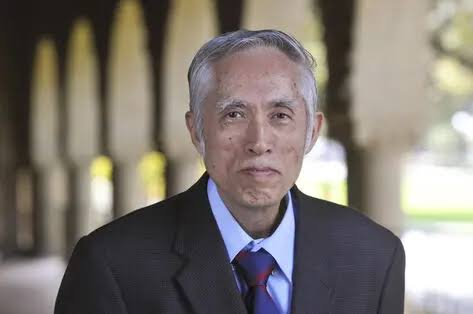
\includegraphics[width=0.6cm,height=0.7cm,keepaspectratio]{images/tzeleunglai.jpg}
      };
      \node[inner sep=0pt] at (-2.92,0.75) {
        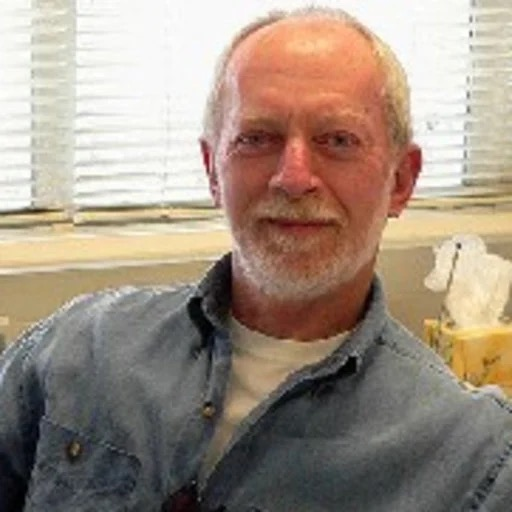
\includegraphics[width=0.6cm,height=0.7cm,keepaspectratio]{images/davidvhinkley.jpg}
      };
      \node[inner sep=0pt] at (-2.27,0.75) {
        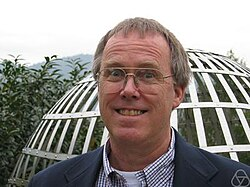
\includegraphics[width=0.6cm,height=0.7cm,keepaspectratio]{images/jamesoberger.jpg}
      };
      \node[inner sep=0pt] at (-1.62,0.75) {
        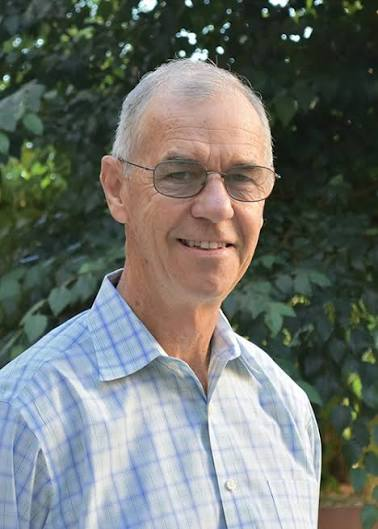
\includegraphics[width=0.6cm,height=0.7cm,keepaspectratio]{images/rosslprentice.jpg}
      };
      \node[inner sep=0pt] at (-0.97,0.75) {
        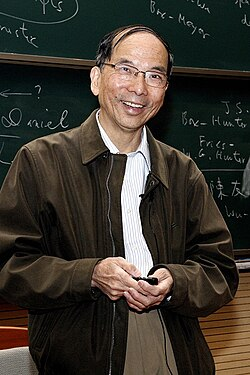
\includegraphics[width=0.6cm,height=0.7cm,keepaspectratio]{images/cfjeffwu.jpg}
      };
      \node[inner sep=0pt] at (-0.33,0.75) {
        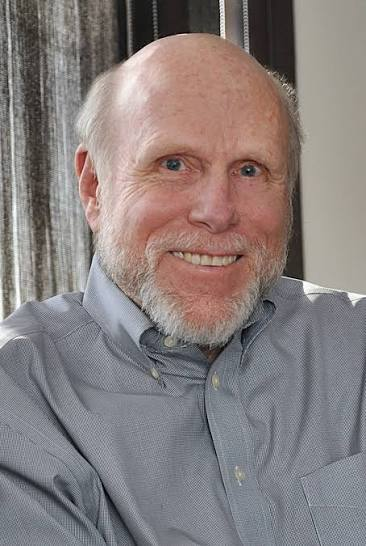
\includegraphics[width=0.6cm,height=0.7cm,keepaspectratio]{images/raymondjcarroll.jpg}
      };
      \node[inner sep=0pt] at (0.33,0.75) {
        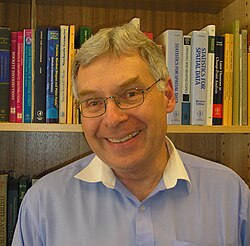
\includegraphics[width=0.6cm,height=0.7cm,keepaspectratio]{images/peterhall.jpg}
      };
      \node[inner sep=0pt] at (0.98,0.75) {
        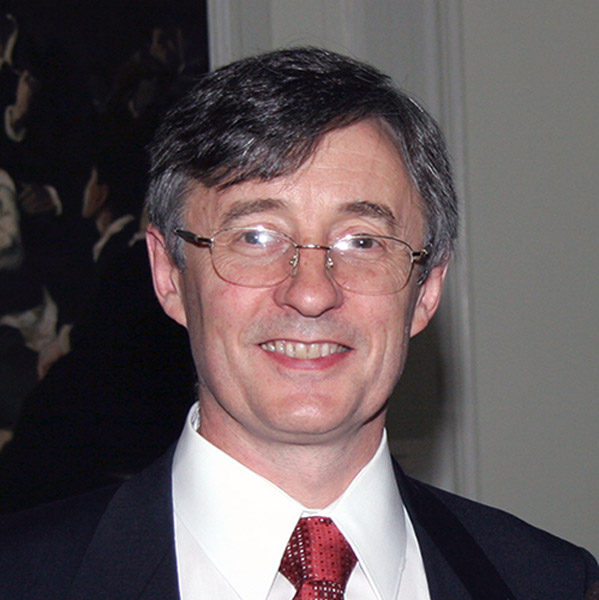
\includegraphics[width=0.6cm,height=0.7cm,keepaspectratio]{images/petermccullagh.jpg}
      };
      \node[inner sep=0pt] at (1.62,0.75) {
        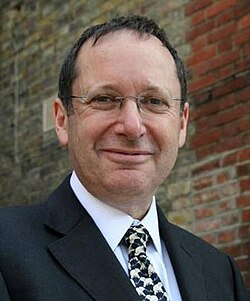
\includegraphics[width=0.6cm,height=0.7cm,keepaspectratio]{images/bernardsilverman.jpg}
      };
      \node[inner sep=0pt] at (2.28,0.75) {
        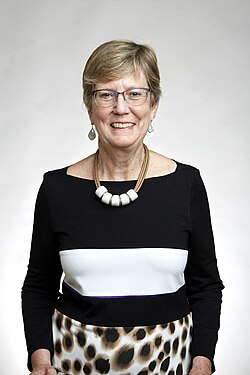
\includegraphics[width=0.6cm,height=0.7cm,keepaspectratio]{images/nancyreid.jpg}
      };
      \node[inner sep=0pt] at (2.93,0.75) {
        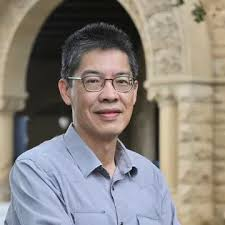
\includegraphics[width=0.6cm,height=0.7cm,keepaspectratio]{images/winghungwong.jpg}
      };
      \node[inner sep=0pt] at (3.58,0.75) {
        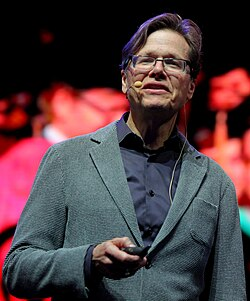
\includegraphics[width=0.6cm,height=0.7cm,keepaspectratio]{images/davidldonoho.jpg}
      };
      \node[inner sep=0pt] at (4.22,0.75) {
        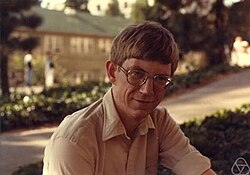
\includegraphics[width=0.6cm,height=0.7cm,keepaspectratio]{images/iainmjohnstone.jpg}
      };
      \node[inner sep=0pt] at (4.88,0.75) {
        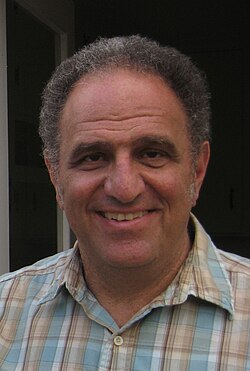
\includegraphics[width=0.6cm,height=0.7cm,keepaspectratio]{images/robertjtibshirani.jpg}
      };
      \node[inner sep=0pt] at (-4.88,0.00) {
        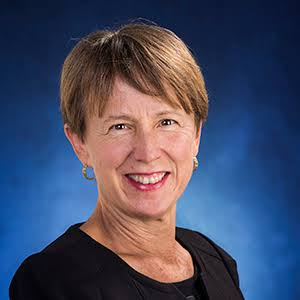
\includegraphics[width=0.6cm,height=0.7cm,keepaspectratio]{images/kathrynroeder.jpg}
      };
      \node[inner sep=0pt] at (-4.22,0.00) {
        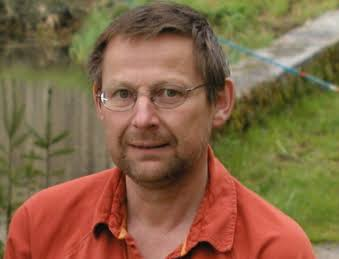
\includegraphics[width=0.6cm,height=0.7cm,keepaspectratio]{images/pascalmassart.jpg}
      };
      \node[inner sep=0pt] at (-3.58,0.00) {
        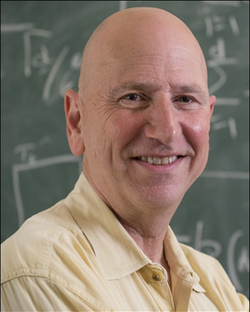
\includegraphics[width=0.6cm,height=0.7cm,keepaspectratio]{images/larryawasserman.png}
      };
      \node[inner sep=0pt] at (-2.92,0.00) {
        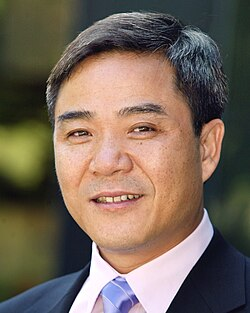
\includegraphics[width=0.6cm,height=0.7cm,keepaspectratio]{images/jianqingfan.jpg}
      };
      \node[inner sep=0pt] at (-2.27,0.00) {
        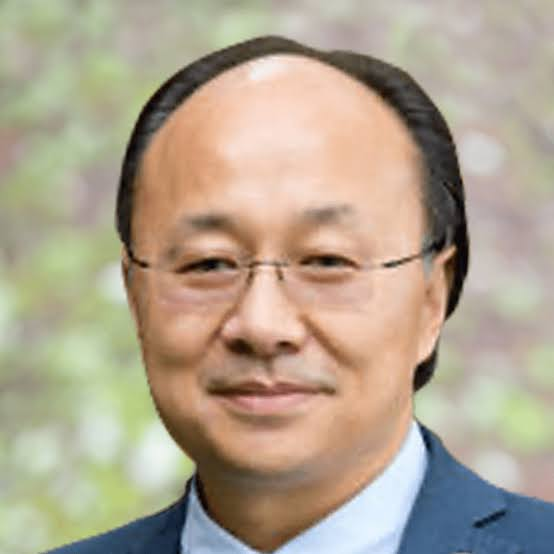
\includegraphics[width=0.6cm,height=0.7cm,keepaspectratio]{images/xiaolimeng.jpg}
      };
      \node[inner sep=0pt] at (-1.62,0.00) {
        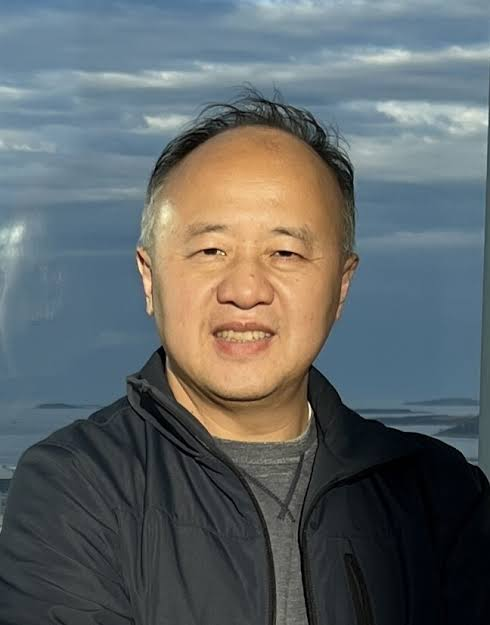
\includegraphics[width=0.6cm,height=0.7cm,keepaspectratio]{images/junliu.jpg}
      };
      \node[inner sep=0pt] at (-0.97,0.00) {
        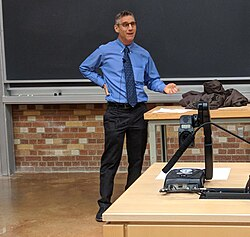
\includegraphics[width=0.6cm,height=0.7cm,keepaspectratio]{images/andrewgelman.jpg}
      };
      \node[inner sep=0pt] at (-0.33,0.00) {
        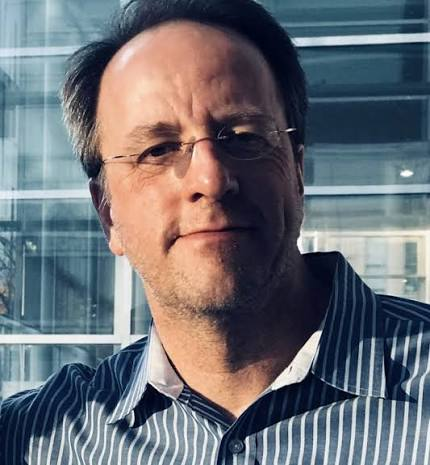
\includegraphics[width=0.6cm,height=0.7cm,keepaspectratio]{images/michaelanewton.jpg}
      };
      \node[inner sep=0pt] at (0.33,0.00) {
        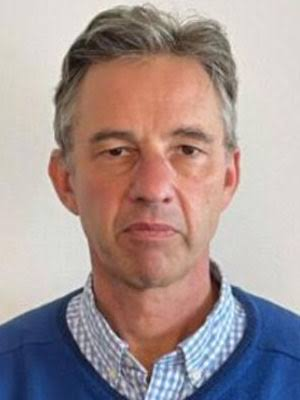
\includegraphics[width=0.6cm,height=0.7cm,keepaspectratio]{images/markjvanderlaan.jpg}
      };
      \node[inner sep=0pt] at (0.98,0.00) {
        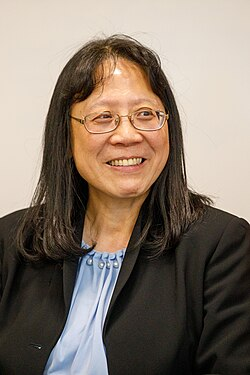
\includegraphics[width=0.6cm,height=0.7cm,keepaspectratio]{images/xihonglin.jpg}
      };
      \node[inner sep=0pt] at (1.62,0.00) {
        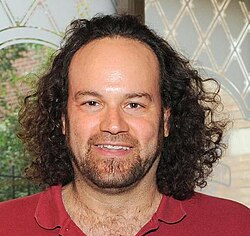
\includegraphics[width=0.6cm,height=0.7cm,keepaspectratio]{images/jeffrosenthal.jpg}
      };
      \node[inner sep=0pt] at (2.28,0.00) {
        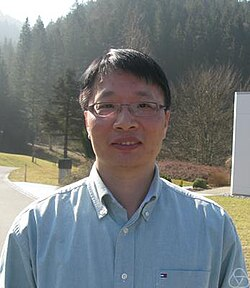
\includegraphics[width=0.6cm,height=0.7cm,keepaspectratio]{images/ttonycai.jpg}
      };
      \node[inner sep=0pt] at (2.93,0.00) {
        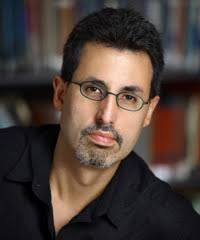
\includegraphics[width=0.6cm,height=0.7cm,keepaspectratio]{images/rafaelirizarry.jpg}
      };
      \node[inner sep=0pt] at (3.58,0.00) {
        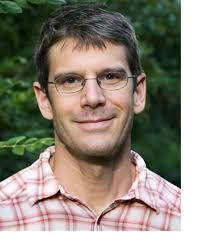
\includegraphics[width=0.6cm,height=0.7cm,keepaspectratio]{images/daviddunson.jpg}
      };
      \node[inner sep=0pt] at (4.22,0.00) {
        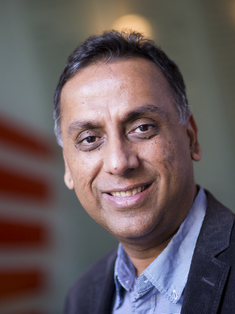
\includegraphics[width=0.6cm,height=0.7cm,keepaspectratio]{images/nilanjanchatterjee.png}
      };
      \node[inner sep=0pt] at (4.88,0.00) {
        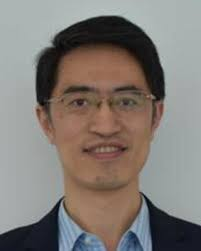
\includegraphics[width=0.6cm,height=0.7cm,keepaspectratio]{images/samuelkou.jpg}
      };
      \node[inner sep=0pt] at (-4.88,-0.75) {
        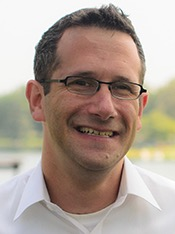
\includegraphics[width=0.6cm,height=0.7cm,keepaspectratio]{images/marcasuchard.jpg}
      };
      \node[inner sep=0pt] at (-4.22,-0.75) {
        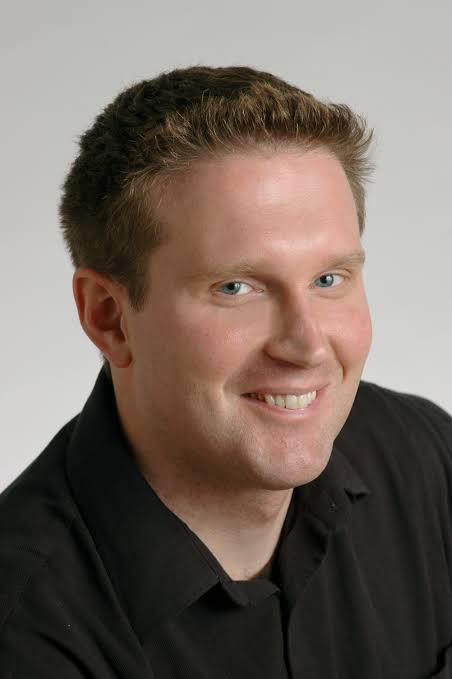
\includegraphics[width=0.6cm,height=0.7cm,keepaspectratio]{images/martinjwainwright.jpg}
      };
      \node[inner sep=0pt] at (-3.58,-0.75) {
        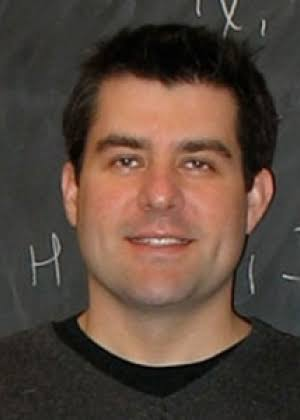
\includegraphics[width=0.6cm,height=0.7cm,keepaspectratio]{images/johndstorey.jpg}
      };
      \node[inner sep=0pt] at (-2.92,-0.75) {
        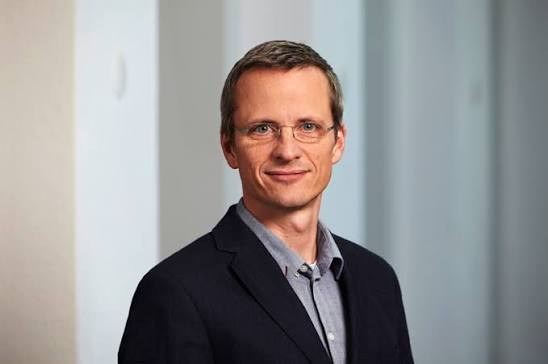
\includegraphics[width=0.6cm,height=0.7cm,keepaspectratio]{images/nicolaimeinshausen.jpg}
      };
      \node[inner sep=0pt] at (-2.27,-0.75) {
        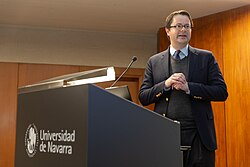
\includegraphics[width=0.6cm,height=0.7cm,keepaspectratio]{images/tylerjvanderweele.jpg}
      };
      \node[inner sep=0pt] at (-1.62,-0.75) {
        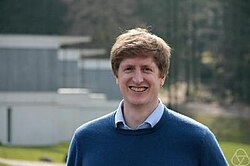
\includegraphics[width=0.6cm,height=0.7cm,keepaspectratio]{images/richardjsamworth.jpg}
      };
      \node[inner sep=0pt] at (-0.97,-0.75) {
        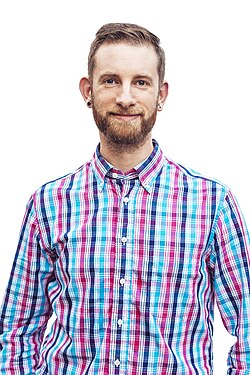
\includegraphics[width=0.6cm,height=0.7cm,keepaspectratio]{images/hadleywickham.jpg}
      };
      \node[inner sep=0pt] at (-0.33,-0.75) {
        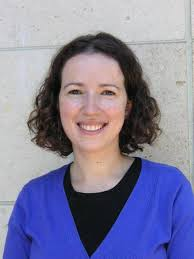
\includegraphics[width=0.6cm,height=0.7cm,keepaspectratio]{images/rinafoygelbarber.jpg}
      };
      \node[inner sep=0pt] at (0.33,-0.75) {
        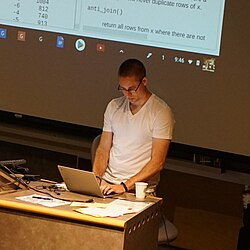
\includegraphics[width=0.6cm,height=0.7cm,keepaspectratio]{images/jeffreytleek.jpg}
      };
      \node[inner sep=0pt] at (0.98,-0.75) {
        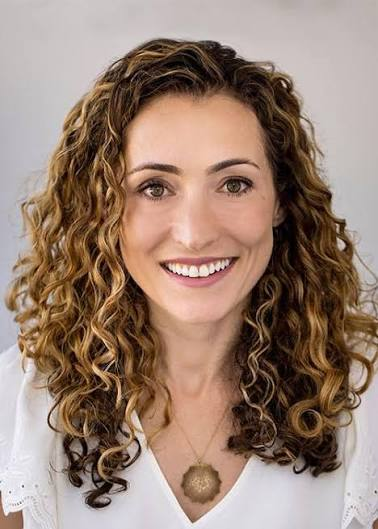
\includegraphics[width=0.6cm,height=0.7cm,keepaspectratio]{images/danielawitten.jpg}
      };
      \node[inner sep=0pt] at (1.62,-0.75) {
        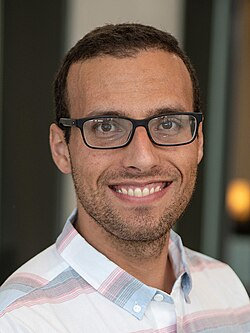
\includegraphics[width=0.6cm,height=0.7cm,keepaspectratio]{images/ryantibshirani.jpg}
      };
      \node[inner sep=0pt] at (2.28,-0.75) {
        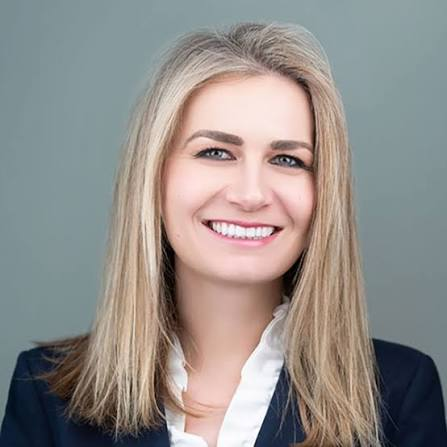
\includegraphics[width=0.6cm,height=0.7cm,keepaspectratio]{images/veronikarockova.jpg}
      };
      \node[inner sep=0pt] at (2.93,-0.75) {
        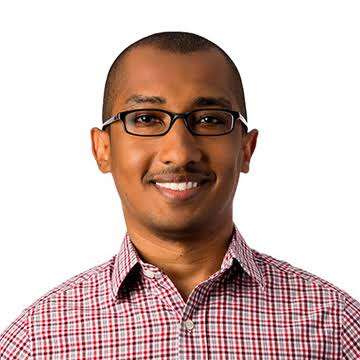
\includegraphics[width=0.6cm,height=0.7cm,keepaspectratio]{images/lestermackey.jpg}
      };
      \node[inner sep=0pt] at (3.58,-0.75) {
        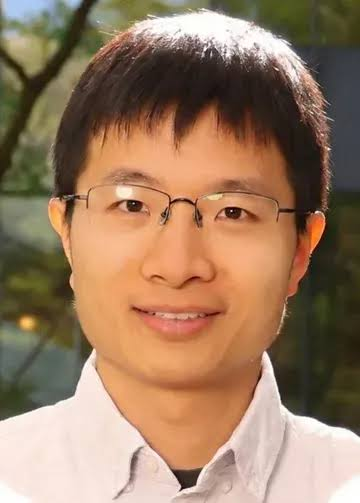
\includegraphics[width=0.6cm,height=0.7cm,keepaspectratio]{images/weijiesu.jpg}
      };
    \end{tikzpicture}
  };
  \node[anchor=south, font=\scriptsize, text=mutedgray]
    at ([yshift=0.38cm]current page.south) {\faIcon{medal}\enspace COPSS Presidents' Award\enspace|\enspace 1981–2026\enspace|\enspace 全 46 位得主};
\end{tikzpicture}
\end{frame}

\def\framesubject{奠基年代}

\begin{frame}{1981–1990}
\vspace{-2pt}
\centering
\scriptsize
\resizebox{\textwidth}{!}{\begin{tabular}{@{}
  >{\raggedright}m{2.55cm}
  >{\centering}m{2.45cm}
  >{\centering}m{2.10cm}
  >{\raggedright}m{1.60cm}
  >{\raggedright}m{2.00cm}
  >{\raggedright\arraybackslash}m{2.40cm}
@{}}
\toprule
\rowcolor{copssbg}
\textbf{姓名} & \textbf{获奖} & \textbf{生卒} & \textbf{国籍} & \textbf{机构} & \textbf{研究领域} \\
\midrule
\lrow{Peter J. Bickel\cn{彼得·比克尔}}{1981（41岁）}{1940–}{美国}{UC Berkeley}{非参数与半参数统计；亦获 MacArthur 1984}
\lrow{Stephen Fienberg\cn{斯蒂芬·费恩伯格}}{1982（40岁）}{1942–2016}{美国}{Carnegie Mellon Univ.}{列联表与社会统计；亦获 R.A. Fisher Lectureship}
\lrow{Tze Leung Lai\cn{黎子良}}{1983（38岁）}{1945–2023}{美国}{Stanford Univ.}{序贯分析与随机逼近}
\lrow{David V. Hinkley\cn{戴维·欣克利}}{1984（40岁）}{1944–2019}{美国}{UC Santa Barbara}{Bootstrap 与渐近理论}
\lrow{James O. Berger\cn{詹姆斯·伯杰}}{1985（35岁）}{1950–}{美国}{Purdue Univ.}{统计决策与贝叶斯；亦获 NAS 2003 · R.A. Fisher Lectureship}
\lrow{Ross L. Prentice\cn{罗斯·普伦蒂斯}}{1986（40岁）}{1946–}{加拿大}{Fred Hutchinson Cancer Research Center}{生存分析与流行病学；亦获 R.A. Fisher Lectureship 2008}
\lrow{C. F. Jeff Wu\cn{吴建福}}{1987（38岁）}{1949–}{美国}{Georgia Institute of Technology}{试验设计与工业统计；亦获 Shewhart Medal · R.A. Fisher Lectureship}
\lrow{Raymond J. Carroll\cn{雷蒙德·卡罗尔}}{1988（39岁）}{1949–}{美国}{Texas A\&M Univ.}{测量误差模型；亦获 R.A. Fisher Lectureship 2002}
\lrow{Peter Hall\cn{彼得·霍尔}}{1989（38岁）}{1951–2016}{澳大利亚}{Australian National Univ.}{非参数统计与 Bootstrap；亦获 Guy Medal 2011 · 澳桂冠学者}
\lrow{Peter McCullagh\cn{彼得·麦卡拉}}{1990（38岁）}{1952–}{美国}{U of Chicago}{广义线性模型；亦获 Guy Medal 金2026 · FRS 1994}
\bottomrule
\end{tabular}}
\vspace{4pt}
\end{frame}

\def\framesubject{贝叶斯复兴与计算革命}

\begin{frame}{1991–2000}
\vspace{-2pt}
\centering
\scriptsize
\resizebox{\textwidth}{!}{\begin{tabular}{@{}
  >{\raggedright}m{2.55cm}
  >{\centering}m{2.45cm}
  >{\centering}m{2.10cm}
  >{\raggedright}m{1.60cm}
  >{\raggedright}m{2.00cm}
  >{\raggedright\arraybackslash}m{2.40cm}
@{}}
\toprule
\rowcolor{copssbg}
\textbf{姓名} & \textbf{获奖} & \textbf{生卒} & \textbf{国籍} & \textbf{机构} & \textbf{研究领域} \\
\midrule
\lrow{Bernard Silverman\cn{伯纳德·西尔弗曼}}{1991（39岁）}{1952–}{英国}{U of Oxford}{密度估计与非参数回归；亦获 Guy Medal · IMO 金牌}
\lrow{Nancy Reid\cn{南希·里德}}{1992（40岁）}{1952–}{加拿大}{U of Toronto}{渐近理论与复合似然}
\lrow{Wing Hung Wong\cn{黄永康}}{1993（41岁）}{1952–}{美国}{Stanford Univ.}{MCMC 与贝叶斯计算}
\lrow{David L. Donoho\gaussbadge\cn{戴维·多诺霍}}{1994（37岁）}{1957–}{美国}{Stanford Univ.}{小波与压缩感知；亦获 ★ Gauss Prize 2018 · Shaw Prize 2013}
\lrow{Iain M. Johnstone\cn{伊恩·约翰斯通}}{1995（39岁）}{1956–}{美国}{Stanford Univ.}{随机矩阵与高维统计；亦获 Guy Medal 银2010}
\lrow{Robert J. Tibshirani\cn{罗伯特·蒂布希拉尼}}{1996（40岁）}{1956–}{美国/加拿大}{Stanford Univ.}{LASSO 与统计学习}
\lrow{Kathryn Roeder\cn{凯瑟琳·罗德}}{1997（37岁）}{1960–}{美国}{Carnegie Mellon Univ.}{统计遗传学与多重检验}
\lrow{Pascal Massart\cn{帕斯卡尔·马萨尔}}{1998（40岁）}{1958–}{法国}{Université de Paris-Sud}{浓度不等式与模型选择}
\lrow{Larry A. Wasserman\cn{拉里·瓦瑟曼}}{1999（40岁）}{1959–}{美国/加拿大}{Carnegie Mellon Univ.}{非参数推断}
\lrow{Jianqing Fan\cn{范剑青}}{2000（38岁）}{1962–}{美国}{Princeton Univ.}{非参数与高维统计；亦获 Guy Medal 银2014 · Guggenheim}
\bottomrule
\end{tabular}}
\vspace{4pt}
\end{frame}

\def\framesubject{生物统计爆发与华人崛起}

\begin{frame}{2001–2010}
\vspace{-2pt}
\centering
\scriptsize
\resizebox{\textwidth}{!}{\begin{tabular}{@{}
  >{\raggedright}m{2.55cm}
  >{\centering}m{2.45cm}
  >{\centering}m{2.10cm}
  >{\raggedright}m{1.60cm}
  >{\raggedright}m{2.00cm}
  >{\raggedright\arraybackslash}m{2.40cm}
@{}}
\toprule
\rowcolor{copssbg}
\textbf{姓名} & \textbf{获奖} & \textbf{生卒} & \textbf{国籍} & \textbf{机构} & \textbf{研究领域} \\
\midrule
\lrow{Xiao-Li Meng\cn{孟晓犁}}{2001（38岁）}{1963–}{美国}{Harvard Univ.}{贝叶斯统计与计算}
\lrow{Jun Liu\cn{刘军}}{2002（37岁）}{1965–}{美国}{Harvard Univ.}{MCMC 与计算生物学}
\lrow{Andrew Gelman\cn{安德鲁·格尔曼}}{2003（38岁）}{1965–}{美国}{Columbia Univ.}{多层次贝叶斯模型}
\lrow{Michael A. Newton\cn{迈克尔·牛顿}}{2004（40岁）}{1964–}{加拿大}{U of Wisconsin}{计算生物学}
\lrow{Mark J. van der Laan\cn{马克·范德兰}}{2005（38岁）}{1967–}{美国}{UC Berkeley}{目标学习与因果推断}
\lrow{Xihong Lin\cn{林希虹}}{2006（40岁）}{1966–}{美国}{Harvard Univ.}{统计遗传学}
\lrow{Jeff Rosenthal\cn{杰夫·罗森塔尔}}{2007（40岁）}{1967–}{加拿大}{U of Toronto}{MCMC 收敛理论}
\lrow{T. Tony Cai\cn{蔡天文}}{2008（41岁）}{1967–}{美国}{U of Pennsylvania}{高维统计推断}
\lrow{Rafael Irizarry\cn{拉斐尔·伊里萨里}}{2009（37岁）}{1972–}{美国}{Harvard Univ.}{基因组数据分析}
\lrow{David Dunson\cn{戴维·邓森}}{2010（38岁）}{1972–}{美国}{Duke Univ.}{贝叶斯非参数}
\bottomrule
\end{tabular}}
\vspace{4pt}
\end{frame}

\def\framesubject{高维统计与机器学习融合}

\begin{frame}{2011–2020}
\vspace{-2pt}
\centering
\scriptsize
\resizebox{\textwidth}{!}{\begin{tabular}{@{}
  >{\raggedright}m{2.55cm}
  >{\centering}m{2.45cm}
  >{\centering}m{2.10cm}
  >{\raggedright}m{1.60cm}
  >{\raggedright}m{2.00cm}
  >{\raggedright\arraybackslash}m{2.40cm}
@{}}
\toprule
\rowcolor{copssbg}
\textbf{姓名} & \textbf{获奖} & \textbf{生卒} & \textbf{国籍} & \textbf{机构} & \textbf{研究领域} \\
\midrule
\lrow{Nilanjan Chatterjee\cn{尼兰詹·查特吉}}{2011（39岁）}{1972–}{美国}{Johns Hopkins Univ.}{统计遗传学与流行病学}
\lrow{Samuel Kou\cn{寇星昌}}{2012（38岁）}{1974–}{美国}{Harvard Univ.}{随机过程与生物物理}
\lrow{Marc A. Suchard\cn{马克·苏查德}}{2013（41岁）}{1972–}{美国}{UCLA}{贝叶斯系统发生学}
\lrow{Martin J. Wainwright\cn{马丁·温赖特}}{2014（41岁）}{1973–}{美国/加拿大}{UC Berkeley}{高维统计与图模型}
\lrow{John D. Storey\cn{约翰·斯托里}}{2015（37岁）}{1978–}{美国}{Princeton Univ.}{多重检验与 q-value}
\lrow{Nicolai Meinshausen\cn{尼古拉·迈因斯豪森}}{2016（38岁）}{1978–}{瑞士/德国}{ETH Zürich}{高维统计与因果}
\lrow{Tyler J. VanderWeele\cn{泰勒·范德维勒}}{2017（40岁）}{1977–}{美国}{Harvard Univ.}{因果中介分析}
\lrow{Richard J. Samworth\cn{理查德·萨姆沃思}}{2018（40岁）}{1978–}{英国}{U of Cambridge}{高维非参数估计}
\lrow{Hadley Wickham\cn{哈德利·威克姆}}{2019（40岁）}{1979–}{新西兰}{RStudio / Posit}{数据科学与可视化}
\lrow{Rina Foygel Barber\cn{里娜·巴伯}}{2020（37/38岁）}{1982/1983–}{美国}{U of Chicago}{选择性推断；亦获 MacArthur 2024}
\bottomrule
\end{tabular}}
\vspace{4pt}
\end{frame}

\def\framesubject{数据科学、AI 与贝叶斯革新}

\begin{frame}{2021–2026}
\vspace{-2pt}
\centering
\scriptsize
\resizebox{\textwidth}{!}{\begin{tabular}{@{}
  >{\raggedright}m{2.55cm}
  >{\centering}m{2.45cm}
  >{\centering}m{2.10cm}
  >{\raggedright}m{1.60cm}
  >{\raggedright}m{2.00cm}
  >{\raggedright\arraybackslash}m{2.40cm}
@{}}
\toprule
\rowcolor{copssbg}
\textbf{姓名} & \textbf{获奖} & \textbf{生卒} & \textbf{国籍} & \textbf{机构} & \textbf{研究领域} \\
\midrule
\lrow{Jeffrey T. Leek\cn{杰弗里·利克}}{2021（41岁）}{1980–}{美国}{Fred Hutchinson Cancer Center}{数据科学与可重复研究}
\lrow{Daniela Witten\cn{丹妮拉·维滕}}{2022（38岁）}{1984–}{美国}{U of Washington}{高维无监督学习}
\lrow{Ryan Tibshirani\cn{瑞安·蒂布希拉尼}}{2023（38岁）}{1985–}{美国/加拿大}{UC Berkeley}{保形预测与分布推断}
\lrow{Veronika Ročková\cn{维罗妮卡·罗奇科娃}}{2024（39岁）}{1985–}{美国}{U of Chicago}{贝叶斯高维模型选择}
\lrow{Lester Mackey\cn{莱斯特·麦基}}{2025（42岁）}{1983–}{美国}{Microsoft Research}{大规模机器学习}
\lrow{Weijie Su\cn{苏炜杰}}{2026（38岁）}{1988–}{美国}{U of Pennsylvania}{深度学习理论}
\bottomrule
\end{tabular}}
\vspace{4pt}
\end{frame}

\def\framesubject{}

\begin{frame}{交叉获奖与荣誉}
\vspace{0.20cm}
\begin{center}
{\Large\bfseries\color{copssclr} COPSS 得主与四大数学奖交叉情况}
\end{center}
\vspace{0.25cm}
{\large
\begin{itemize}\setlength\itemsep{14pt}\setlength\leftmargin{0.6cm}
  \item[\textcolor{fieldsclr}{$\blacklozenge$}] \textbf{菲尔兹 / 沃尔夫 / 阿贝尔 / 陈省身奖章}：46 位 COPSS 得主中 \textbf{无人} 同时获得（统计学与纯数学领域不同，2026 年为止）。
  \item[\textcolor{wolfclr}{$\bigstar$}] \textbf{David L. Donoho（1994）}：另获 \textbf{IMU 高斯奖 2018}（应用数学最高荣誉）与 \textbf{邵逸夫奖 2013}——COPSS 得主中与数学界奖项交叉最显著者。
  \item[\textcolor{copssclr}{$\blacklozenge$}] \textbf{统计领域荣誉交叉}：R.A. Fisher Lectureship（9 人）；Guy 奖章（6 人）；MacArthur 天才奖（Bickel 1984·Barber 2024）。
\end{itemize}
}
\end{frame}

\end{document}
